\achapter{16}{Quotient Spaces}\label{chap:quotients}


\vspace*{-17 pt}
\framebox{
\parbox{\dimexpr\linewidth-3\fboxsep-3\fboxrule}
{\begin{fqs}
\item What is a quotient topology?
\item What is a quotient space?
\item What are two examples of familiar quotient spaces?
\end{fqs}}}

\vspace*{13 pt}

\csection{Introduction}\label{sec_quotients}

We are familiar with the word \emph{quotient} when working with rational numbers. That is, the fraction $\frac{1}{2}$ is the quotient of $1$ by $2$, and the set of rational numbers is the collection of all defined quotients of integers. The word quotient seems to have come from the latin word ``quotiens", which can be translated as ``how often" or ``how many times". We can think of the fraction $\frac{1}{2}$ as dividing a unit ($1)$ into two pieces. So we often apply the word quotient to any kind of construction that divides a set into pieces. Another familiar quotient construction is the set $\Z_n$, the set of quotients of integers after we divide by $n$. Another way to think of $\Z_n$ is as a quotient $\Z/n\Z$, where $n\Z$ is the set of multiples of $n$ and two integers $a$ and $b$ are equal if $b-a \in n\Z$. This defines the relation of congruence module $n$ on $\Z$, and the elements of $\Z/n\Z$ are the equivalence classes for this relation. We make similar constructions in many branches of mathematics by defining an equivalence relation on a set, and we then divide the set into pieces (the equivalence classes) and call the set of equivalence classes a \emph{quotient space}. We explore the concept of quotient spaces of topological spaces in this section.

As an example, take the interval $X = [0,1]$ in $\R$ and bend it to be able to glue the endpoints together. The resulting object is a circle. By identifying the endpoints $0$ and $1$ of the interval, we are able to create a new topological space. We can view this gluing or identifying of points in the space $X$ in a formal way that allows us to recognize the resulting space as a quotient space. 

\csection{The Quotient Topology}\label{sec_quotient_top}

Given a topological space $X$ and a surjection $f$ from $X$ to a set $Y$, we can use the topology on $X$ to define a topology on $Y$. This topology on $Y$ identifies points in $X$ through the function $f$. The resulting topology on $Y$ is called a \emph{quotient} topology. The quotient topology gives us a way of creating a topological space which models gluing and collapsing parts of a topological space.

\begin{pa} Let $X = \{1,2,3,4,5,6\}$ and let $\tau = \{\emptyset, \{1,2\},\{4,6\}, \{1,2,4,6\},X\}$. Let $Y = \{a,b,c,d\}$ and define $p: X \to Y$ by 
\[p(1) = b, \ p(2) = a, \ p(3) = c, \ p(4) = d, \ p(5) = c, \ \text{ and } \ p(6) = a.\] 
Our goal in this activity is to define a topology on $Y$ that is related to the topology on $X$ via $p$. 
\be
\item We know the sets in $X$ that are open. So let us consider the sets $U$ in $Y$ such that $p^{-1}(U)$ is open in $X$. Define $\sigma$ to be this set. That is
\[\sigma = \{U \subseteq Y \mid p^{-1}(U) \in \tau\}.\]
Find all of the sets in $\sigma$. 

\item Show that $\sigma$ is a topology on $Y$.

\item Explain why $p : (X, \tau) \to (Y, \sigma)$ is continuous.

\item Show that $\sigma$ is the largest topology on $Y$ for which $p$ is continuous. That is, if $\sigma'$ is a topology on $Y$ with $\sigma \subsetneqq \sigma'$, then $p: (X,\tau) \to (Y, \sigma')$ is not continuous.

\ee

\end{pa}

\begin{comment}

\ActivitySolution

\be
\item The only possibilities for sets $U$ are those with $p^{-1}(U)$ being $\emptyset$, $\{1,2\}$, $\{4,6\}$, $\{1,2,4,6\}$, and $X$. Since $p$ is a surjection, the only time $p^{-1}(U) = \emptyset$ is when $U = \emptyset$. Also, $p^{-1}(U) = X$ when $X = Y$. We consider the remaining cases in turn. 

\begin{itemize}
\item Since $p(1) = p(6) = b$ and $p(2) = a$, $p^{-1}(U)$ can never be  $\{1,2\}$.
\item Since $p(4) = d$, and $p(2) = p(6) = a$, $p^{-1}(U)$ can never be $\{4,6\}$. 
\item Since $p(1) = b$, $p(2) = p(6) = a$, and $p(4) = d$, $p^{-1}(U) = \{1,2,4,6\}$ when $U = \{a,b,d\}$. 
\end{itemize}
Thus, 
\[\sigma = \{\emptyset, \{a,b,d\}, Y\}.\]

\item By inspection we can see that unions and intersections of sets in $\sigma$ remain in $\sigma$, so $\sigma$ is a topology on $Y$.  

\item By definition, if $U$ is in $\sigma$, then $p^{-1}(U)$ is in $\tau$. So the inverse image of any open set is open under $p$ and $p$ is continuous.

\item Suppose $\sigma'$ is a topology on $Y$ with $\sigma \subset \sigma'$. Then there exists $O \in \sigma' \setminus \sigma$. If $p^{-1}(O)$ were open, then we would have $O \in \sigma$ be definition. But this is a contradiction. So $p^{-1}(O)$ is not open and $p$ is not continuous from $(X \tau)$ to $(Y, \sigma')$. 

\ea

\end{comment}

\csection{Quotient Spaces}\label{sec_quotient_space}

As we saw in our preview activity, if we have a surjection $p$ from a topological space $(X,\tau)$ to a set $Y$, we were able to define a topology on $Y$ by making the open sets the sets $U \subseteq Y$ such that $p^{-1}(U)$ is open in $X$. This is how we will create what is called the \emph{quotient topology}.  Before we can define the quotient topology, we need to know that this construction always makes a topology.

\begin{activity} \label{act:quot_topology} Let $(X,\tau_X)$ be a topological space, let $Y$ be a set, and let $p: X \to Y$ be a surjection. Let 
\[\tau_Y = \{U \subseteq Y \mid p^{-1}(U) \in \tau_X\}.\]
\ba
\item Why are $\emptyset$ and $Y$ in $\tau_Y$?

\item Let $\left\{U_{\beta}\right\}$ be a collection of sets in $\tau_Y$ for $\beta$ in some indexing set $J$. 
	\begin{enumerate}[i.]
	\item Show that $\bigcup_{\beta \in J} U_{\beta}$ is in $\tau_Y$.
	
	\item If $J$ is finite, show that $\bigcap_{\beta \in J} U_{\beta}$ is in $\tau_Y$.
	
	\end{enumerate}
	
\item What conclusion can we draw about $\tau_Y$? 

\ea

\end{activity}

\begin{comment}

\ActivitySolution

\ba
\item Since $p^{-1}(\emptyset) = \emptyset \in \tau_X$ we have that $\emptyset \in \tau_Y$. The fact that $p$ is a surjection means that $p^{-1}(Y) = X \in \tau_X$. So $Y \in \tau_Y$.

\item Let $\left\{U_{\beta}\right\}$ be a collection of sets in $\tau_Y$ for $\beta$ in some indexing set $J$. 
	\begin{enumerate}[i.]
	\item By definition, $p^{-1}(U_{\beta} \in \tau_X$ for every $\beta \in J$. Since $p^{-1}\left(\bigcup_{\beta \in J} U_{\beta}\right) = \bigcup_{\beta \in J} p^{-1}\left(U_{\alpha}\right)$ is in $\tau_X$ it follows that $\bigcup_{\beta \in J} U_{\beta}$ is in $\tau_Y$.
	
	\item Since $p^{-1}\left(\bigcap_{\beta \in J} U_{\beta}\right) = \bigcap_{\beta \in J} p^{-1}\left(U_{\alpha}\right)$ is in $\tau_X$ it follows that $\bigcap_{\beta \in J} U_{\beta}$ is in $\tau_Y$.
	
	\end{enumerate}
	
\item We can conclude that $\tau_Y$ is a topology on $Y$. 

\ea

\end{comment}

Activity \ref{act:quot_topology} allows us to define the quotient topology.

\begin{definition} Let $(X,\tau_X)$ be a topological space, let $Y$ be a set, and let $p: X \to Y$ be a surjection. 
\begin{enumerate}
\item The \textbf{quotient topology}\index{quotient topology} on $Y$ is the set
\[\{U \subseteq Y \mid p^{-1}(U) \in \tau_X\}.\]
\item Any function $p: X \to Y$ is a \textbf{quotient map}\index{quotient map} if $p$ is surjective and for $U \subseteq Y$,  $U$ is open in $Y$ if and only if $p^{-1}(U)$ is open in $X$. 
\item If $p: X \to Y$ is a quotient map, then the space $Y$ is the \textbf{quotient space}\index{quotient space} of $X$ determined by $p$. 
\end{enumerate}
\end{definition}


\begin{activity} ~
\ba
\item Let $X=\R$ with standard topology, let $Y=\{-1,0,1\}$, and define $p:X \to Y$ by 
\[p(x) = \begin{cases} 1&\text{if } x>0 \\ 0 &\text{if } x=0 \\ -1 &\text{if } x<0. \end{cases}\]
Find all of the open sets in the quotient topology. 

\item Let $X=\R$ with standard topology, let $Y=[0,1)$, and define $p:X \to Y$ by 
\[p(x) = x-\lfloor x\rfloor,\]
where $\lfloor x\rfloor$ is the largest integer less than or equal to $x$, (For example $\lfloor 1.2 \rfloor = 1$, and so $p(1.2) = 1.2 - 1 = 0.2$. The function defined by $\lfloor x\rfloor$ is also called the \emph{floor} function. Be careful, note that $\lfloor -0.7 \rfloor = -1$.)  Determine the sets in the quotient topology.  (Hint: The graph of $p$ on $[-2,2]$ is shown in Figure \ref{F:floor}.)
\begin{figure}[h]
\begin{center}
\resizebox{!}{1.0in}{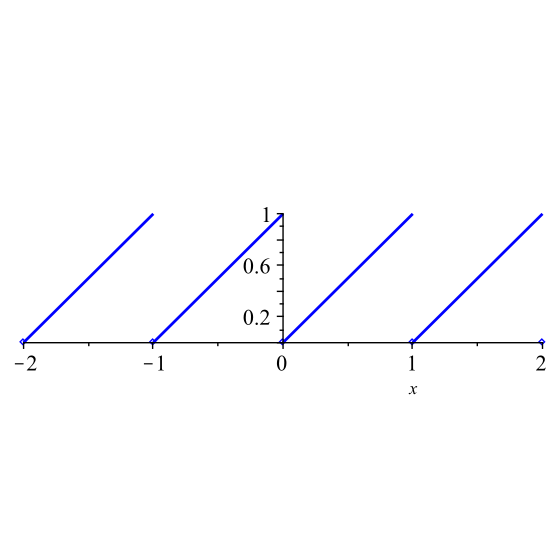
\includegraphics[trim=0.75cm 6.5cm 0.75cm 6.75cm, clip]{floor.eps}}
\caption{The graph of $p(x) = x - \lfloor x\rfloor$.} 
\label{F:floor}
\end{center}
\end{figure}
%\includegraphics[trim=left bottom right top, clip]{file}


\ea

\end{activity}

\begin{comment}

\ActivitySolution
\ba
\item We know that $\emptyset$ and $Y$ are open. We consider all of the remaining subsets of $Y$. Note that 
\begin{align*}
p^{-1}(\{-1\}) &= (-\infty, 0), \\
p^{-1}(\{0\}) &= \{0\}, \\
p^{-1}(\{1\}) &= (0,\infty, 0), \\
p^{-1}(\{-1,0\}) &= (-\infty, 0], \\
p^{-1}(\{-1,1\}) &= (-\infty, 0) \cup (0, \infty), \text{ and } \\
p^{-1}(\{0,1\}) &= [0,\infty).
\end{align*}
The only subsets of $Y$ that have open inverse images are $\{-1\}$, $\{1\}$, and $\{-1,1\}$. So the quotient topology is
\[\{\emptyset, \{-1\}, \{1\}, \{-1,1\}, Y\}.\]

\item The graph shows that for $y$ in $Y$, we have 
\[p^{-1}(y) = \{k+y \mid k \in \Z\}.\]
So $p^{-1}(B) = \{k+b \mid k \in \Z \text{ and } b \in B\}$. The only way for $p^{-1}(B)$ to be open in $X$ is for $p^{-1}(B)$ to be a union of open intervals. This will happen only when $B$ is a union of open intervals in $Y$. Since $p^{-1}((a,b)) = \bigcup_{k \in \Z} (k+a, k+b)$ when $0 \leq a < b < 1$, the quotient topology is 
\[\{\emptyset,Y\} \cup \{(a,b) \mid 0 \leq a < b < 1\}.\]


\ea

\end{comment}

Another perspective of the quotient topology utilizes the fact that any equivalence relation on a set $X$ partitions $X$ into a union of disjoint equivalence classes $[x] = \{y \in X \mid y \sim x\}$. There is a natural surjection $q$ from $X$ to the space of equivalence classes given by $q(x) = [x]$. We investigate this perspective in the next activity.

\begin{activity} \label{act:quotient_er} Let $X = \{a,b,c,d,e,f\}$ and let $\tau = \{\emptyset, \{a\}, \{b\}, \{a, b\}, \{a, b, c\}, \{a, b, c, d\}, X\}$. Then $(X, \tau)$ is a topological space. Let $A = \{a, b, c\}$ and $B = \{d,e,f\}$. Define a relation $\sim$ on $X$ such that $x \sim y$ if $x$ and $y$ are both in $A$ or both in $B$. Assume that $\sim$ is an equivalence relation. The sets $A$ and $B$ are the equivalence classes for this relation. That is $A = [a] = [b] = [c]$ and $B = [d] = [e] = [f]$. Let $X^* = \{A,B\}$. Then we can define $p : X \to X^*$ by sending $x \in X$ to the set to which it belongs. That is, $p(x) = [x]$ for $x \in X$, or 
\[p(a) = A, p(b) = A, p(c) = A, p(d) = B, p(e) = B, \text{ and } p(f) = B.\]
Determine the sets in the quotient topology on $X^*$. 
\end{activity}

\begin{comment}

\ActivitySolution Since $X^{*} = \{A,B\}$, there are only limited possibilities for open sets. We consider each in turn: 
\begin{align*}
p^{-1}(\emptyset) &= \emptyset \\
p^{-1}(\{A\}) &= \{a,b,c\} \\
p^{-1}(\{B\}) &= \{d,e,f\} \\
p^{-1}(X^{*}) &= X.
\end{align*}
From this list we see that the quotient topology on $X^{*}$ is $\{\emptyset, \{A\}, X^{*}\}$. 

\end{comment}

The partition of $X$ in Activity \ref{act:quotient_er} into the disjoint union of sets $A$ and $B$ defines an equivalence relation on $X$ where $x \sim y$ if $x$ and $y$ are both in the same set $A$ or $B$. That is, $a \sim b \sim c$ and $d \sim e \sim f$. In this context, the sets $A$ and $B$ are equivalence classes -- $A = [a]$ and $B = [d]$, where $[x]$ is the equivalence class of $x$. This leads to a general construction.

If $(X, \tau)$ is a topological space and $\sim$ is an equivalence relation on $X$, we can let $X/\ssim$ be the set of distinct equivalence classes of $X$ under $\sim$. Then $p: X \to X/\ssim$ defined by $p(x) = [x]$ is a surjection and $X/\ssim$ has the quotient topology. The space $X/\ssim$ is called a \emph{quotient space}\index{quotient space}. The space $X/\ssim$ is also called an \emph{identification} space\index{identification space} because the equivalence relation identifies points in the set to be thought of as the same. This allows us to visualize quotient spaces as resulting from gluing or collapsing parts of the space $X$.

\begin{figure}[h]
\begin{center}
\resizebox{!}{0.75in}{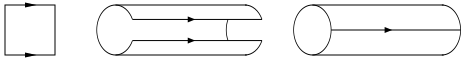
\includegraphics{Cylinder_identification.eps}} 
\caption{A tube as the identification space $X/\ssim$.} 
\label{F:Quotient_tube}
\end{center}
\end{figure}
%\includegraphics[trim=left bottom right top, clip]{file}

\begin{example} Let $I = [0,1]$ and let $X = I \times I$ with standard topology. Define a relation $\sim$ on $X$ by $(x,y) \sim (x,y)$ if $0 < y < 1$ and $0 \leq x \leq 1$, $(x,0) \sim (x,1)$ if $0 \leq x \leq 1$. It is straightforward to show that $\sim$ is an equivalence relation. Let us consider what the identification space $X/\ssim$ looks like. The space $I \times I$ is the unit square as shown in Figure \ref{F:Quotient_tube}. All points in the interior of the square are identified only with themselves. However, the top side and bottom side are identified with each other in the same direction. Think of $X$ as a piece of paper. We roll up the sides of the square to make the top and bottom sides coincide. The result is that $X/\ssim$ is the cylinder as shown in Figure \ref{F:Quotient_tube}. 

\end{example}

\begin{activity} Quotient spaces can be difficult to describe. This activity presents a few more examples. 
\ba
\item Let $X = [0, 1]$ with standard topology and define an equivalence relation $\sim$ on $X$ by $0 \sim 1$ and $x \sim x$ for all $x$ not equal to $0$ or $1$. What does the quotient space $X/\ssim$ look like? (Hint: Think about the relation $\sim$ as gluing the points $0$ and $1$ together.)

\begin{figure}[h]
\begin{center}
\resizebox{!}{1.0in}{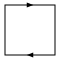
\includegraphics{Mobius_identification.eps}} \hspace{0.5in} \resizebox{!}{1.0in}{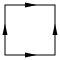
\includegraphics{Torus_identification.eps}} \hspace{0.5in} \resizebox{!}{1.0in}{
\includegraphics[trim=1.8cm 4.0cm 1.25cm 4.7cm, clip]{Quotient_sphere_1.png}} 
\caption{From left to right: the identifications for parts i., ii., and iii.} 
\label{F:Quotients_activity}
\end{center}
\end{figure}

\item Describe quotient spaces of $X = I \times I$ with standard topology given by the following equivalence relations $\sim$. Depictions of the identifications are shown in Figure \ref{F:Quotients_activity}. (Here $I$ is the closed interval $[0,1]$.)
	\begin{enumerate}[i.]
	\item $(x, y) \sim (x,y)$ if $0 < y < 1$ and $0 \leq x \leq 1$ and $(x,0) \sim (1-x,0)$ when $0 \leq x \leq 1$. 
	
	\item $(x, y) \sim (x,y)$ if $0 < x < 1$ and $0 < y < 1$, $(x,0) \sim (x,1)$ for $0 < x < 1$, $(0,y) \sim (1,y)$ for $0 < y < 1$, and $(0,0) \sim (0,1) \sim (1,0) \sim(1,1)$
	
	\item  $(x, y) \sim (x,y)$ if $0 < x < 1$ and $0 < y < 1$ and $(x,y) \sim (u,v)$ if $(x,y)$ and $(u,v)$ are boundary points.
	
	\end{enumerate}
	
\ea

\end{activity}

\begin{comment}

\ActivitySolution

\ba
\item If we take the unit interval $X$ and glue the points $0$ and $1$ together, we obtain a circle, that is the space $S^1$. 

\item Describe quotient spaces of $X = I \times I$ with standard topology given by the following equivalence relations $\sim$. (Here $I$ is the closed interval $[0,1]$.)
	\begin{enumerate}[i.]	
	\item All points in the interior of the square are identified only with themselves. However, the top side and bottom side are identified with each other -- but in the opposite direction as indicated at left in Figure \ref{F:Quotient_Mobius}. So if we roll up and twist the square to make the top and bottom sides coincide in the opposite direction, we obtain the M\"{o}bius strip as shown at right in Figure \ref{F:Quotient_Mobius}.
\begin{figure}[h]
\begin{center}
\resizebox{!}{1.25in}{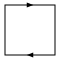
\includegraphics{Mobius_identification.eps}} \hspace{0.75in} \resizebox{!}{1.25in}{\includegraphics[trim=10.75cm 9.05cm 9.9cm 16.25cm, clip]{Mobius.png}} 
\caption{A M\"{o}bius strip as the identification space $X/\ssim$.} 
\label{F:Quotient_Mobius}
\end{center}
\end{figure}
%\includegraphics[trim=left bottom right top, clip]{file}	

	
	\item All points in the interior of the square are identified only with themselves. However, the left side and right side are identified with each other, as are the top and bottom -- both in the same direction as indicated in Figure \ref{F:Quotient_tube}. So if we first roll up the square to identify the left and right sides, we obtain a cylinder. The top and bottom of the square become the top and bottom of the cylinder. Now bend the cylinder around to identify the top and bottom, resulting in the torus as shown at right in Figure \ref{F:Quotient_torus} (image copied from \url{http://i.stack.imgur.com/FJaFe.png}). . 
\begin{figure}[h]
\begin{center}
\resizebox{!}{0.75in}{\includegraphics{Quotient_torus_2.pdf}} 
\caption{A torus as the identification space $X/\ssim$.} 
\label{F:Quotient_torus}
\end{center}
\end{figure}
%\includegraphics[trim=left bottom right top, clip]{file}	

	\item  All points in the interior of the square are identified only with themselves, but the boundaries points are all identified together as indicated at left in Figure \ref{F:Quotient_sphere}. So the boundary collapses to a point. Think of taking the square and pinching all of the sides together. What is left looks like a sphere, with the sides all identified with a single point on the sphere as shown at right in Figure \ref{F:Quotient_sphere}. %Note: An illustration of this can be seen at \url{https://upload.wikimedia.org/wikipedia/commons/4/44/Disk_to_Sphere_using_Quotient_Space.gif}.
\begin{figure}[h]
\begin{center}
\resizebox{!}{1.25in}{
\includegraphics[trim=1.8cm 4.0cm 1.25cm 4.7cm, clip]{Quotient_sphere_1.png}} \hspace{0.75in} \resizebox{!}{1.25in}{\includegraphics[trim=3.2cm 2.3cm 3.0cm 3.1cm, clip]{Quotient_sphere_2.png}} 
\caption{A sphere as the identification space $X/\ssim$.} 
\label{F:Quotient_sphere}
\end{center}
\end{figure}
%\includegraphics[trim=left bottom right top, clip]{file}	

	\end{enumerate}
	
\ea

\end{comment}

Many other interesting identification spaces can be made. For example, let $X = I \times I$ and define $\sim$ by $(x, y) \sim (x,y)$ if $0 < x < 1$ and $0 < y < 1$, $(0, y) \sim (1, y)$ for $0 < y < 1$, $(x,0) \sim (1-x,1)$ for $0 < x < 1$. This identification is illustrated in Figure \ref{F:Klein_bottle}. The resulting identification space $X/\ssim$ is a Klein bottle. A nice illustration of this can be seen at 
\url{https://plus.maths.org/content/introducing-klein-bottle}.
\begin{figure}[h]
\begin{center}
\resizebox{!}{1.25in}{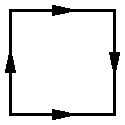
\includegraphics{Klein_identification.eps}} 
\caption{Identifications for the Klein Bottle.} 
\label{F:Klein_bottle}
\end{center}
\end{figure}

\csection{Identifying Quotient Spaces}\label{sec_find_quotient_space}

Suppose $X$ is a topological space and $Y$ is a set, and let $p: X \to Y$ be a surjection. We can define a relation $\sim_p$ on $X$ by $x \sim_P y$ if and only if $p(x) = p(y)$. It is straightforward to show that $\sim_p$ is an equivalence relation. From this we can see that our two approaches to defining the quotient topology and quotient spaces are really the same. 

Oftentimes we have a topological space $X$ and a relation $\sim$ on $X$, and we would like to have an effective way to be able to identify the quotient space $X/\ssim$ as homeomorphic to some familiar topological space $Y$. That is, we want to be able to show that there is a homeomorphism $f$ from $X/\ssim$ to $Y$. 

\begin{example} \label{exp:R_Z_quotient} Consider the following situation. Let $X = \R$ with the standard topology and define the relation $\sim$ on $\R$ by $x \sim y$ if $x - y \in \Z$. It is straightforward to show that $\sim$ is an equivalence relation. By this equivalence relation, we have $x-1 \sim x$ for every real number $x$. This identifies $\R$ with the interval $[0,1]$, where $0$ and $1$ are identified under the relation. So we might expect that $\R/\ssim$ is homeomorphic to the circle $S^1 = \{(x,y) \in \R^2 \mid x^2+y^2 = 1\}$ as a subspace of $\R^2$ with the standard topology. Now the objective is to find a homeomorphism between $S_1$ and $\R/\ssim$. Since every point on the unit circle has the form $(\cos(t), \sin(t))$ for some real number $t$, we might try defining $f: (\R/\ssim) \to S^1$ by $f([t]) = (\cos(t), \sin(t))$. However, we have that $0 \sim 1$, which means that $[0] = [1]$, but $f([0]) \neq f([1])$ and so $f$ is not well-defined. Another option might be $f([t]) = (\cos(2 \pi t), \sin(2 \pi t))$. In this case, if $x \sim y$, then $2 \pi x$ and $2 \pi y$ differ by a multiple of $2 \pi$ and so $f([x]) = f([y])$. We could then show that $f$ is a homeomorphism. We will continue this example shortly.

\end{example}

The following theorem encapsulates the above example.

\begin{theorem} \label{thm:quotient_1} Let $X$ and $Y$ be sets and let $\sim$ be an equivalence relation on $X$. Let $f$ be a function from $X$ to $Y$ such that $f(x_1) = f(x_2)$ whenever $x_1 \sim x_2$ in $X$. Let $X/\ssim$ be the set of equivalence classes of $X$ under the relation $\sim$, and let $p: X \to (X/\ssim)$ be the standard map defined by $p(x) = [x]$.  The function $\overline{f}$ mapping $X/\ssim$ to $Y$ defined by $\overline{f}([x]) = f(x)$ for every $x \in X$ is the unique function that satisfies 
\[f = \overline{f} \circ p.\]
\end{theorem}


\begin{activity} Theorem \ref{thm:quotient_1} is a statement about sets and functions, and there is no topology involved. We prove the theorem in this activity. Use the conditions stated in Theorem \ref{thm:quotient_1}.
\ba
\item Show that $\overline{f}$ is well-defined. That is, show that whenever $[x_1] = [x_2]$ in $X/\ssim$, then $\overline{f}([x_1]) =\overline{f}([x_2])$.

\item Prove that $f = \overline{f} \circ p$. 

\item Show that the uniqueness of $\overline{f}$ comes from the equation $f = \overline{f} \circ p$.

\ea

\end{activity}

\begin{comment}

\ActivitySolution

\ba
\item The fact that $f(x_1) = f(x_2)$ whenever $x_1 \sim x_2$ in $X$ makes $\overline{f}$ well-defined. That is, if $[x_1] = [x_2]$ in $X/\ssim$, then $x_1 \sim x_2$ and so 
\[\overline{f}([x_1]) = f(x_1) = f(x_2) = \overline{f}([x_2]).\]

\item To demonstrate that $f = \overline{f} \circ p$, let $x \in  X$. Then 
\[(\overline{f} \circ p)(x) = \overline{f}(p(x)) = \overline{f}([x]) = f(x).\]

\item For uniqueness, if $g : (X/\ssim) \to Y$ satisfies $g \circ p = f$, then $g(p(x)) = g([x]) = f(x)$ for every $x \in X$ and $g = \overline{f}$.

\ea

\end{comment}

Now we present a final result that can be very helpful when working with quotient spaces.

\begin{theorem} \label{thm:quotient_2} Let $X$ be a topological space and let $\sim$ be an equivalence relation on $X$. Consider the set $X/\ssim$ to be a topological space with the quotient topology, and let $p: X \to (X/\ssim)$ be the standard surjection defined by $p(x) = [x]$. Let $Y$ be a topological space with $f: X \to Y$ a continuous function such that $f(x_1) = f(x_2)$ whenever $x_1 \sim x_2$ in $X$. Then $\overline{f} : (X/\ssim) \to Y$ defined by $\overline{f}([x]) = f(x)$ is the unique continuous function satisfying $f = \overline{f} \circ p$.
\end{theorem}

\begin{proof} The existence of $\overline{f}$ as the unique function satisfying $f = \overline{f} \circ p$ was established in Theorem \ref{thm:quotient_1}. All that remains is to show that $\overline{f}$ is continuous. Let $O$ be an open set in $Y$. Since $f$ is continuous, we know that $f^{-1}(O)$ is open in $X$. If $x_1 \in f^{-1}(O)$ and $x_1 \sim x_2$, then $x_2 \in f^{-1}(O)$ as well. Thus, we can write $f^{-1}(O)$ as
\[f^{-1}(O) = \bigcup_{x \in f^{-1}(O)} [x].\]
That is, $f^{-1}(O)$ is a union of equivalence classes. Now $\overline{f}([x]) = f(x)$, so if $x \in f^{-1}(O)$, then $[x] \in \overline{f}^{-1}(O)$. Thus,
\[f^{-1}(O) = \bigcup_{x \in f^{-1}(O)} [x] = \bigcup_{[x] \in \overline{f}^{-1}(O)} [x] = \overline{f}^{-1}(O).\]
We conclude that $\overline{f}^{-1}(O)$ is open in $X$ and $\overline{f}$ is continuous. 
\end{proof}

Now we will see how to use Theorem \ref{thm:quotient_2} to establish a homeomorphism from a quotient space of a given topological space to another topological space

\begin{example} We return to the situation from Example \ref{exp:R_Z_quotient} with $X = \R$ under the standard topology and equivalence relation $\sim$ defined by $x \sim y$ if $x - y \in \Z$. We will use Theorem \ref{thm:quotient_2} to show that $\R/\ssim$ is homeomorphic to the circle $Y = S^1$. 

\begin{figure}[h]
\begin{center}
\resizebox{!}{1.5in}{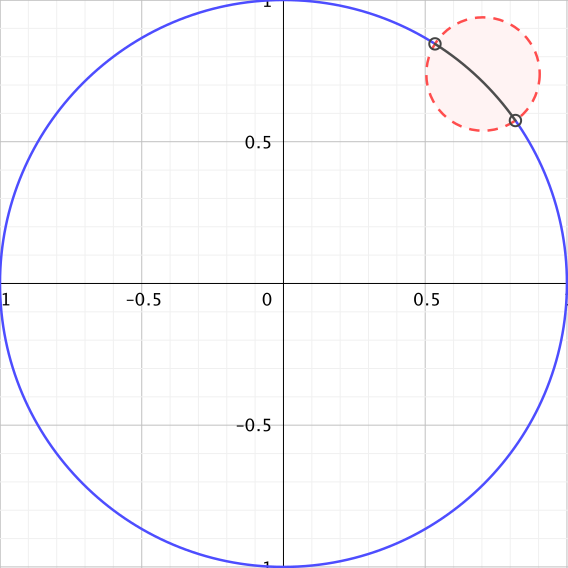
\includegraphics{S_1_basis.eps}} 
\caption{A basis element for $S^1$.} 
\label{F:S_1_basis}
\end{center}
\end{figure}
%\includegraphics[trim=left bottom right top, clip]{file}


\begin{description}
\item[Step 1.] Define a continuous surjection $f: X \to Y$ that respects the relation. That is, we need to ensure that $f(x_1) = f(x_2)$ whenever $x_1 \sim x_2$ in $X$. We saw earlier that the function $f$ defined by $f(t) = (\cos(2 \pi t), \sin(2 \pi t))$ respects the relation. Since every point on the unit circle is of the form $(\cos(\theta), \sin(\theta))$ for some real number $\theta$, choosing $t = \frac{\theta}{2 \pi}$ makes $f(t) = (\cos(\theta), \sin(\theta))$ and $f$ is a surjection. Now we need to demonstrate that $f$ is continuous. A collection of basic open sets in $S^1$ can be found by intersecting $S^1$ with open balls in $\R^2$ as illustrated in Figure \ref{F:S_1_basis}. We can see that the basic open sets are arcs of the form $\wideparen{ab}$ for $a$ and $b$ in $S^1$. Suppose $a = (\cos(2 \pi A), \sin(2 \pi A))$ and $b = (\cos(2 \pi B), \sin(2 \pi B))$ for angles $A$ and $B$. Then $f^{-1}(\wideparen{ab})$ is the union of intervals $(A+2\pi k, B+2 \pi k)$ for $k \in \Z$. As a union of open intervals, we have that $f^{-1}(\wideparen{ab})$ is open in $X$. We have now found a continuous surjection from $X$ to $Y$ that respects the relation. 

\item[Step 2.] Find a continuous function from $X/\ssim$ to $Y$. Theorem \ref{thm:quotient_2} tells us that the function $\overline{f} : (X/\ssim) \to Y$ defined by $\overline{f}([t]) = f(t)$ is continuous. So $\overline{f}$ is our candidate to be a homeomorphism. 

\item[Step 3.] Show that $\overline{f}$ is a bijection. Let $y \in Y$. The fact that $f$ is a surjection means that there is a $t \in \R$ such that $f(t) = y$. It follows that $\overline{f}([t]) = f(t) = y$ and $\overline{f}$ is a surjection. To demonstrate that $\overline{f}$ is an injection, suppose $\overline{f}([s]) = \overline{f}([t])$ for some $s, t \in \R$.  Then $(\cos(2 \pi s), \sin(2 \pi s)) = f(s) = f(t) = (\cos(2\pi t), \sin(2 \pi t))$. It must be the case then that $2 \pi s$ and $2 \pi t$ differ by a multiple of $2 \pi$. That is, $2 \pi s - 2 \pi t = 2 \pi k$ for some integer $k$. From this we have $s - t = k \in \Z$, and so $s \sim t$. This makes $[s] = [t]$ and we conclude that $\overline{f}$ is an injection. 

\item[Step 4.] Show that $\overline{f}$ is a homeomorphism. At this point we already know that $\overline{f}$ is a continuous bijection, so the only item that remains is to show that $\overline{f}(\overline{O})$ is open whenever $\overline{O}$ is open in $X/\ssim$. Let $p: X \to (X/\ssim)$ be the standard map. Let $\overline{O}$ be a nonempty open set in $X/\ssim$. Then $O = p^{-1}(\overline{O})$ is open in $X$. Thus, $O$ is a union of open intervals. Let $(a,b)$ be an interval contained in $O$. From the definition of $f$ we have that $f(a,b)$ is the open arc $\wideparen{f(a)f(b)}$, which is open in $Y$. So $f(O)$ is a union of open arcs in $Y$, which makes $f(O)$ open in $Y$. Now $f(O) = (\overline{f} \circ p)(O) = \overline{f}(p(O)) = \overline{f}(\overline{O})$, and $\overline{f}(\overline{O})$ is open in $Y$. We conclude that $\overline{f}$ is a homeomorphism from $X/\ssim$ to $S^1$, and so $S^1$ is a quotient space of $\R$. 
\end{description}

\end{example}





\csection{Summary}\label{sec_quotients_summ}
Important ideas that we discussed in this section include the following.
\begin{itemize}
\item Let $(X,\tau_X)$ be a topological space, let $Y$ be a set, and let $p: X \to Y$ be a surjection. The quotient topology on $Y$ is the set
\[\{U \subseteq Y \mid p^{-1}(U) \in \tau_X\}.\]
\item The function $p$ is a quotient topology as in the previous bullet is called a quotient map and the space $Y$ is a quotient space. 
\item A circle, a M\"{o}bius strip, a torus, and a sphere can all be realized as quotient spaces. 
\end{itemize}

\csection{Exercises}\label{sec_quotients_exer}

\be

\item Let $X$ be the real numbers with the standard topology and let $p: X \to \{a,b,c\}$ be defined by 
\[p(x) = \begin{cases} a &\text{ if } x < 0 \\ b &\text{ if } x = 0 \\ c &\text{ if } x > 0. \end{cases}\]
What is the quotient topology? 

\begin{comment}

\ExerciseSolution A subset $U$ of $\{a,b,c\}$ is in the quotient topology if and only if $p^{-1}(U)$ is open in $X$. Now 
\begin{align*}
p^{-1}(\{a\}) &= (-\infty, 0) \\
p^{-1}(\{b\}) &= \{0\} \\
p^{-1}(\{c\}) &= (0, \infty) \\
p^{-1}(\{a,b\}) &= (-\infty, 0] \\
p^{-1}(\{a,c\}) &= (-\infty, 0) \cup (0, \infty) \\
p^{-1}(\{b,c\}) &= [0,\infty),
\end{align*}
so the quotient topology is $\{\emptyset, \{a\}, \{c\}, \{a,c\}, \{a,b,c\}\}$.  

\end{comment}

\item Define an equivalence relation $\sim$ on $\R^2$ by $(x_1,y_1) \sim (x_2,y_2)$ whenever $x_2 - x_1 \in \Z$ and $y_2 - y_1 \in \Z$. 

\ba

\item Prove that $\sim$ is an equivalence relation on $\R^2$.

\item The quotient space is a familiar space. Find that space and explain why it is the quotient space.

\ea

\begin{comment}

\ExerciseSolution 

\ba

\item Let $(x_1,y_1)$, $(x_2, y_2)$, and $(x_3,y_3)$ be in $\R^2$. Since $x_1 - x_1 = 0 = y_1 - y_1$ we see that $(x_1,y_1) \sim (x_1, y_1)$ and $\sim$ is reflexive.

Now suppose that $(x_1,y_1) \sim (x_2,y_2)$. Then $x_2 - x_1 \in \Z$ and $y_2 - y_1 \in \Z$. So $x_1 - x_2 = -(x_2-x_1) \in \Z$ and $y_1-y_2 = -(y_2 - y_1) \in \Z$. Thus, $(x_2, y_2) \sim (x_1,y_1)$ and $\sim$ is symmetric.

Finally, suppose that $(x_1,y_1) \sim (x_2,y_2)$ and $(x_2,y_2) \sim (x_3,y_3)$. Then $x_3-x_1 = (x_3-x_2) + (x_2-x_1) \in \Z$ and $(y_3-y_1) = (y_3-y_2) + (y_2-y_1) \in \Z$ and $\sim$ is transitive. Therefore, $\sim$ is an equivalence relation. 

\item Let $A = \{(x,y) \mid 0 \leq x < 1, 0 \leq y < 1\}$. If $u \in \R$, then $u$ has a decimal expansion $u = u_0.u_1u_2 \ldots$, where $u_0 \in \Z$. Let $u' = 0.u_1u_2 \ldots$. Then $u - u' \ldots = u_0$. So $u \sim u'$ and $0 \leq u' < 1$. From this we can say that any $(u,v) \in \R^2$ is equivalent to a point $(u',v') \in A$. Now if $(x,y)$ and $(r,s)$ are points in $A$, then $0 \leq |x-r| < 1$ and $0 \leq |y-s| < 1$. So $(x,y) \not\sim (r,s)$ if $(x,y) \neq (r,s)$. Therefore, the set $A$ contains representatives of all of the distinct equivalence classes, with one representative for each point. Because $(1,y) \sim (0,y)$ for each $y$ and $(x,1) \sim (x,0)$ for each $x$, the opposite boundaries of $A$ are identified. So the quotient space is the torus. 

\ea

\end{comment}

\item Find an example of a continuous surjection that is not a quotient map.

\begin{comment}

\ExerciseSolution Let $X$ be the reals with the discrete topology and $Y$ the reals with the standard Euclidean topology. Define $p : X \to Y$ by $p(x) = x$. Then $p$ is a continuous surjection, but $\{0\} = p^{-1}(\{0\})$ is open in $X$ even though $\{0\}$ is not open in $Y$.  

\end{comment}


\item Let $X$ be a topological space and let $A$ be a subspace of $X$. Define a relation $\sim$ on $X$ whose equivalence classes are $A$ and $\{x\}$ if $x \notin A$. In this case the quotient space is denoted as $X/A$ (think of this space as obtained by crushing $A$ to a point and leaving everything else alone). Describe each of the following quotient spaces.
\ba

\item  $X$ is the closed interval $[0,1]$ in $\R$ and $A = \{0,1\}$

\item $X = \{(x,y) \mid x^2+y^2 = 1\}$, $A = \{(-1,0), (1,0)\}$

\item If $X= \{(x,y) \mid x^2+y^2 \leq 1\}$ and $A = \{(x,y) \mid x^2+y^2 = 1\}$

\ea


\begin{comment}

\ExerciseSolution

\ba

\item This space identifies the endpoints of the unit interval and we have seen that this quotient space is a circle.

\item Take a circle and smash two antipodal points together and we get a figure eight.

\item If we identify all of the points on the boundary of a disk we end up with the surface of a sphere. 

\ea

\end{comment}

\item Let $(X, \tau)$ be the topological space where $X = \{1, 2, 3, 4\}$ and 
\[\tau = \{\emptyset, \{1\}, \{2\}, \{1, 2\}, \{3, 4\}, \{2, 3, 4\}, \{1, 3, 4\}, \{1, 2, 3, 4\}\}.\]
Let $Y = \{a, b, c\}$.
\ba
\item Let $p: X \to Y$ be defined by $p(1)=a$, $p(2) = a$, $p(3)=b$, and $p(4) = c$. Find the quotient topology $\tau_p$ on $Y$ defined by the function $p$.

\item Let $q : X \to Y$ be defined by $q(1)=c$, $q(2) = c$, $q(3) = b$, and $q(4) = a$. Find the quotient topology $\tau_q$ on $Y$ defined by the function $q$.

\item Are the spaces $(Y, \tau_p)$ and $(Y, \tau_q)$ homeomorphic? If yes, write down a specific homeomorphism and explain why your mapping is a homeomorphism. If not, explain why not.

\ea

\begin{comment}

\ExerciseSolution

\ba
\item Since 
\begin{align*}
p^{-1}(\{a\}) &= \{1,2\} \in \tau \\
p^{-1}(\{b\}) &= \{3\} \notin \tau \\
p^{-1}(\{c\}) &= \{4\} \notin \tau \\
p^{-1}(\{a,b\}) &= \{1,2,3\} \notin \tau \\
p^{-1}(\{a,c\}) &= \{1,2,4\} \notin \tau \\
p^{-1}(\{b,c\}) &= \{3,4\} \in \tau,
\end{align*}
we have that $\tau_p = \{\emptyset, \{a\}, \{b,c\}, Y\}$. 

\[\tau = \{\emptyset, \{1\}, \{2\}, \{1, 2\}, \{3, 4\}, \{2, 3, 4\}, \{1, 3, 4\}, \{1, 2, 3, 4\}\}.\]
Let $Y = \{a, b, c\}$.
\item Since 
\begin{align*}
q^{-1}(\{a\}) &= \{4\} \notin \tau \\
q^{-1}(\{b\}) &= \{3\} \notin \tau \\
q^{-1}(\{c\}) &= \{1,2\} \in \tau \\
q^{-1}(\{a,b\}) &= \{3,4\} \in \tau \\
q^{-1}(\{a,c\}) &= \{1,2,4\} \notin \tau \\
q^{-1}(\{b,c\}) &= \{1,2,3\} \notin \tau,
\end{align*}
we have that $\tau_q = \{\emptyset, \{c\}, \{a,b\}, Y\}$. 

\item Define $f : Y \to Y$ by $f(a) = c$, $f(b) = a$, and $f(c) = b$. Note that $f$ is a bijection by construction. Since 
\[f^{-1}(\{c\}) = \{a\} \ \text{ and } \ f^{-1}(\{a,b\}) = \{b,c\}\]
we see that the inverse image of every open set is an open set. So $f$ is continuous. Also,
\[f(\{a\}) = \{c\} \ \text{ and } \ f(\{b,c\}) = \{a,b\},\]
and the image of every open set is open. So $f^{-1}$ is continuous. We conclude that $f$ is a homeomorphism and that $(Y, \tau_p)$ and $(Y, \tau_q)$ are homeomorphic spaces. 

\ea


\end{comment}

\item Let $D^2 = \{(x,y) \in \R^2 \mid x^2+y^2 \leq 1\}$ be the unit disk in $\R^2$ with the standard topology, and let $S^1 = \{(x,y) \mid x^2+y^2 = 1\}$ be the boundary of $D^2$. Describe the quotient spaces $D^2/\ssim$ for each equivalence relation (assume that points are similar to themselves). Let $x = (s_1,t_1)$ and $y = (s_2,t_2)$. 

\ba
\item $x \sim y$ if $s_1=s_2$ for $x, y$ in $D^2$

\item $x \sim y$ if $s_1=s_2$ for $x, y$ in $S^1$

\item $x \sim y$ if $x$ and $y$ are diagonally opposite each other for $x, y$ in $D^2$

\ea


\begin{comment}

\ExerciseSolution

\ba

\item This is the line segment $[-1,1]$.

\item This is like a cylinder, but with closed ends. Think of a calzone that has no filling.

\item Every line through the origin has two equivalent parts - the points on the line above the $y$-axis are equivalent to the corresponding points on the line below the $y$-axis. So we can think of the space $D^2/\ssim$ as the upper half disk consisting of the line segments from the origin to points on $S^1$. 


\ea

\end{comment}

\item Let $X = I \times I$ where $I$ is the interval $[0,1]$ with the standard metric topology, and define an equivalence relation on $X$ by $(s_1, t_1) \sim (s_2,t_2)$ when $t_1 = t_2 > 0$ and $x \sim x$ for all other $x \in X$. 
\ba
\item Describe the quotient space $X/\ssim$, and describe the quotient topology.

\item Show that $X/\ssim$ is not Hausdorff.

\ea

\begin{comment}

\ExerciseSolution

\ba

\item The identification $(s_1, t_1) \sim (s_2,t_2)$ when $t_1 = t_2 > 0$ collapses all bu the bottom edge of $X$ to a half open line segment of the form $(0,1]$. So $X/\ssim$ can be thought of as a horizontal line segment $K = [0,1]$ with a line segment $J = (0,1]$ attached vertically. The subsets of $J$ whose inverse images are open sets are the open subintervals of $J$. The subsets of $K$ whose inverse images are open sets are the open intervals in $K$ along with open intervals in $J$ of the form $(0,r)$, where $r$ is the radius of the given interval, as illustrated in Figure \ref{F:Quotient_Homework_Segments}.  
\begin{figure}[h]
\begin{center}
\resizebox{!}{1.0in}{\includegraphics{Quotient_Homework_Segments.eps}}
\caption{The quotient space.} 
\label{F:Quotient_Homework_Segments}
\end{center}
\end{figure}
%\includegraphics[trim=left bottom right top, clip]{file}

\item If $a$ and $b$ are points in $K$, then any open sets $O_a$ and $O_b$ containing $a$ and $b$ also contain an open interval in $J$. So it is impossible to separate two points in $K$ with open sets in $X/\ssim$ and so $X/\ssim$ is not Hausdorff. 

\ea

\end{comment}

\item Let $X$ be a nonempty set and let $p$ be a fixed element in $X$. Let $\tau_p$ be the particular point topology and $\tau_{\overline{p}}$ the excluded point topology on $X$. That is
\begin{itemize}
\item $\tau_{p}$ is the collection of subsets of $X$ consisting of $\emptyset$, $X$, and all of the subsets of $X$ that contain $p$.  
\item $\tau_{\overline{p}}$ is the collection of subsets of $X$ consisting of $\emptyset$, $X$, and all of the subsets of $X$ that do not contain $p$.
\end{itemize}
That the particular point and excluded point topologies are topologies is the subject of Exercises (\ref{ex:particular_point_topology}) and (\ref{ex:excluded_point_topology}) on page \pageref{ex:particular_point_topology}. 

Let $\sim$ be the equivalence relation on $\Z$ defined by $x \sim y$ if $x \equiv y \pmod{3}$. Describe the quotient space $\Z/\ssim$ and then determine, with justification, the quotient topology on $\Z/\ssim$ when
	\ba
		
	\item $\Z$ has the topology $\tau_{p}$ with $p = 1$
	
	\item $\Z$ has the topology $\tau_{\tau_{\overline{p}}}$ with $p = 1$.		
	
	\ea
	
\begin{comment}

\ExerciseSolution The quotient space $\Z/\ssim$ is the set of congruence classes in $\Z_3$. That is, $(\Z/\ssim) = \{[0], [1], [2]\}$. Let $f: \Z \to \Z/\ssim$ be defined by $f(n) = [n]$.
	\ba
	\item We find the inverse images of all subsets of $\Z/\ssim$:
		\begin{itemize}
		\item $f^{-1}(\emptyset) = \emptyset$
		\item $f^{-1}(\{[0]\}) = \{n \in \Z \mid n = 3k \text{ for some } k \in \Z\}$
		\item $f^{-1}(\{[1]\}) = \{n \in \Z \mid n = 3k+1 \text{ for some } k \in \Z\}$
		\item $f^{-1}(\{[2]\}) = \{n \in \Z \mid n = 3k+2 \text{ for some } k \in \Z\}$
		\item $f^{-1}(\{[0],[1]\}) = \{n \in \Z \mid n = 3k \text{ or } n = 3k+1 \text{ for some } k \in \Z\}$
		\item $f^{-1}(\{[0],[2]\}) = \{n \in \Z \mid n = 3k \text{ or } n = 3k+2 \text{ for some } k \in \Z\}$
		\item $f^{-1}(\{[1],[2]\}) = \{n \in \Z \mid n = 3k+1 \text{ or } n = 3k+2 \text{ for some } k \in \Z\}$
		\item $f^{-1}(\Z/\ssim) = \Z$.
		\end{itemize}
The inverse images that are open are the empty set and the sets that contain $p=1$. So the quotient topology is 
\[\{\emptyset, \{[1]\}, \{[0], [1]\}, \{[1], [2]\}, \Z/\ssim\}.\]

	\item We have the same quotient space and the same inverse images. The inverse images that are open sets now are the empty set and the sets that don't contain $p=1$. So the quotient topology is
\[\{\emptyset, \{[0]\}, \{[2]\}, \{[0], [2]\},  \Z/\ssim\}.\]
	
	\ea


\end{comment}


\item In the process of developing techniques of drawing in perspective, renaissance artists found it necessary to consider a point at infinity where all lines intersect. This creates a geometry that extends the concept of the real plane. This new geometry is the real projective plane $\mathbb{R}P^2$\index{real projective plane}, which can be thought of as the quotient space of $\R^3 \setminus \{(0,0,0)\}$ with the relation $\sim_P$ such that $(x_1,x_2,x_3) \sim_P (y_1,y_2,y_3)$ in $\R^3 \setminus \{(0,0,0)\}$ if and only if there is a nonzero real number $k$ such that $y_1 = kx_1$, $y_2 = kx_2$, and $y_3 = kx_3$.  In the projective plane, parallel lines intersect at a point at infinity, just as they seem to with our human vision. 

\ba

\item Show that $\sim_P$ is an equivalence relation.

\item Give a geometric description of the elements in the quotient space $\mathbb{R}P^2$.  

\item There are other ways to visualize $\mathbb{R}P^2$. For example, explain why the real projective plane $\mathbb{R}P^2$ is homeomorphic to the quotient space $S^2/\ssim$ of $S^2 = \{(x,y,z) \in \R^3 \mid x^2+y^2+z^2 = 1\}$, where $\sim$ identifies antipodal points on $S^2$. No formal proofs are necessary, but a convincing explanation is in order.

\item Since we identify antipodal points on $S^2$ in the space $S^2/\sim$, we can think of this space in another way. If $P$ is a point on $S^2$ not on the equator, then its antipodal point is also not on the equator. So we can think of $S^2/\ssim$ as the top hemisphere, along with the equator on which antipodal points are identified, as illustrated at left in Figure \ref{F:projective_1}. 
\begin{center}
\begin{figure}[h]
\begin{center}
\resizebox{!}{1.25in}{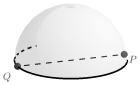
\includegraphics[trim=3.55cm 3.75cm 3.55cm 3.0cm, clip]{projective_1.png}} \hspace{0.25in} \resizebox{!}{1.25in}{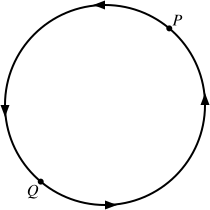
\includegraphics{Projective_disk.eps}} \hspace{0.25in} \resizebox{!}{1.25in}{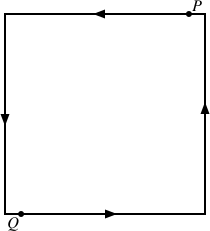
\includegraphics{Projective_square.eps}}
\caption{Three perspectives of $\mathbb{R}P^2$.} 
\label{F:projective_1}
\end{center}
\end{figure}
\end{center}
%\includegraphics[trim=left bottom right top, clip]{file}
By projecting the points on the hemisphere down to the $xy$-plane, we can represent $S^2/\ssim$ as a disk whose antipodal points are identified, as seen in the middle in Figure \ref{F:projective_1}. Use this last perspective to explain why $\mathbb{R}P^2$ can be realized as a square where opposite sides are identified in opposite directions as shown at right in Figure \ref{F:projective_1}.

\item The projective plane $\mathbb{R}P^2$ is a complicated object -- it cannot be embedded in $\R^3$ and so it is not something that can be easily visualized. The projective plane is a non-orientable surface and is also important in classifying surfaces -- basically, every closed surface is made up of spheres, tori, and/or projective planes. In this part of the exercise we see how the projective plane itself is made by adjoining a M{\"o}bius strip to a disk (think of sewing the boundary of M{\"o}bius strip to the perimeter of a disk). 
	\begin{enumerate}[i.]
	
	\item Start with the model of $\mathbb{R}P^2$ shown at left in Figure \ref{F:projective_2}. Partition this object into three pieces as shown at right in Figure \ref{F:projective_2}. Explain why the shaded region in the middle figure, separated out at right in Figure \ref{F:projective_2}, is a M{\"o}bius strip. 

\begin{center}
\begin{figure}[h]
\begin{center}
\resizebox{!}{1.25in}{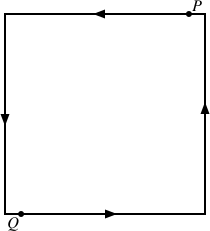
\includegraphics{Projective_square.eps}} \hspace{0.25in} \resizebox{!}{1.25in}{\includegraphics{Projective_Mobius.eps}} \hspace{0.25in} \begin{minipage}{0.75in} {\vspace{-1.0in} \resizebox{!}{0.75in}{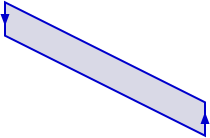
\includegraphics{Projective_Mobius_split.eps}}} \end{minipage}
\caption{Splitting the real projective plane.} 
\label{F:projective_2}
\end{center}
\end{figure}
\end{center}

	\item The space $S$ that remains after we remove the M{\"o}bius strip from $\mathbb{R}P^2$ is shown at left in Figure \ref{F:projective_3}. The two spaces that follow are homeomorphic to $S$. Describe the homeomorphisms that produce the spaces from $S$. Then explain how $\mathbf{R}P^2$ is obtained by attaching a M{\"o}bius strip to a disk along its boundary. 
\begin{center}
\begin{figure}
\begin{center}
\resizebox{!}{1.25in}{\includegraphics{Projective_Disk_split.eps}} \hspace{0.1in} \begin{minipage}[c]{0.25in}{\vspace{-1.25in} $\xrightarrow{f}$}\end{minipage} \hspace{0.1in} \resizebox{!}{1.25in} {\includegraphics{Projective_Disk_hom_1.eps}} \hspace{0.1in} \begin{minipage}[c]{0.25in}{\vspace{-1.25in} $\xrightarrow{g}$}\end{minipage} \hspace{0.1in} \resizebox{!}{1.25in}{\includegraphics{Projective_Disk_hom_2.eps}}
\caption{Recognizing the space $S$.} 
\label{F:projective_3}
\end{center}
\end{figure}
\end{center}
	\end{enumerate}

\ea

\begin{comment}

\ExerciseSolution

\ba

\item Let $x = (x_1,x_2,x_3)$, $y = (y_1,y_2,y_3)$, and $z = (z_1,z_2, z_3)$ be in $\R^3 \setminus \{(0,0,0)\}$. Since $x_i = x_i$ for each $i$, we see that $x \sim_P x$ and so $\sim_P$ is reflexive.

Suppose that $x \sim_P y$. Then $y_1 = kx_1$, $y_2 = kx_2$, and $y_3 = kx_3$ for some nonzero constant $k$. Then $x_i = \frac{1}{k} y_i$ for each $i$ and $y \sim_P x$. So $\sim_P$ is symmetric. 

Finally, suppose that $x \sim_P y$ and $y \sim_P z$. Then $y_i = kx_i$ and $z_i = my_i$ for nonzero constants $k$ and $m$ for each $i$. Thus, $z_i = my_i = (mk) x_i$ for each $i$ and $x \sim_P z$. Thus, $\sim_P$ is transitive and is an equivalence relation.

\item The graph of the set of equations $y_1 = kx_1$, $y_2 = kx_2$, and $y_3 = kx_3$ is the line in $\R^3$ through the origin and the point $(x_1, x_2, x_3)$. So these lines minus the origin form the elements of $\mathbb{R}P^2$.

\item Let $P$ be a point on $S^2$ and let $\ell_P$ be the line through the origin and $P$. If we let $[P]$ denote the equivalence class of point $P$ under $\sim$ that identifies antipodal points, then the mapping $f: S_2/\ssim \to \mathbb{R}P^2$ defined by $f([P]) = \ell_P$ is a bijection and, ultimately, a homeomorphism.

\item Starting with the disk, we can stretch the points on the disk out toward the square as illustrated in Figure \ref{F:disk_to_square}. This stretching provides a homeomorphism from the disk to the square.
\begin{center}
\begin{figure}[h]
\begin{center}
\resizebox{!}{0.75in}{\includegraphics{Disk_to_square_1.eps}} \hspace{0.2in} \resizebox{!}{0.75in} {\includegraphics{Disk_to_square_2.eps}} \hspace{0.2in} \resizebox{!}{0.75in} {\includegraphics{Disk_to_square_3.eps}} \hspace{0.2in} \resizebox{!}{0.75in} {\includegraphics{Disk_to_square_4.eps}}
\caption{Stretching the disk to the square.} 
\label{F:disk_to_square}
\end{center}
\end{figure}
\end{center}

\item Reflect the bottom figure about the $c$-axis. Then reflect the top figure about its $c$-axis, and reflect again around its $b$-axis. Finally translate the two figures so that their $c$-axes coincide. This provides the homeomorphism $f$. The homeomorphism $g$ is the identification mapping which identifies the two segments $a$ and the two segments $b$. The mapping $g$ also rotates the identified segments $a$ and $b$ to align them with segment $c$, then stretches segments $x$ and $y$ to semicircles. The result is that $S$ is homeomorphic to a disk. Notice that the boundary of the disk matches the boundary of the M{\"o}bius strip that was removed. So if we sew the M{\"o}bius strip on to the disk along the boundary, we will return to $\mathbb{R}P^2$. 

\ea

\end{comment}

\item Let $X = \R^2$ with the standard topology, and let $Y = \{x \in \R \mid x \geq 0\}$ with the standard topology. Let $f: X \to Y$ be defined by $f((x,y)) = x^2+y^2$. 
\ba
\item Show that $f$ is a continuous surjective function.

\item Prove that the quotient space $X^{*}$ of $X$ defined by $f$ is homeomorphic to $Y$.

\ea


\begin{comment}

\ExerciseSolution 

\ba

\item First notice that if $r$ is greater than or equal to $0$, $f$ maps the circle of radius $r$ onto $r$. So $f$ is a surjection. Also, if $r^2 \in Y$, then $f^{-1}(r^2) = \{(x,y) \mid x^2+y^2 = r^2\}$. So $f^{-1}(r^2)$ is the circle centered at the origin with radius $r$. Let $a$ and $b$ be in $Y$ with $a < b$. Then $f^{-1}((a,b))$ is the open region between the circles of radii $\sqrt{a}$ and $\sqrt{b}$. So $(a,b)$ is open in $Y$. It is also the case that $f^{-1}([0,b))$ is the open ball centered at $0$ of radius $\sqrt{b}$. So $f^{-1}([0,b))$ is open in $Y$. So $f$ is continuous.  

\item If $(x,y)$ is in $\R^2$ with $x^2+y^2 = r^2$, the equivalence class $[(x,y)]$ is the set $\{(u,v) \in \R^2 \mid u^2+v^2 = r^2\}$. That is, $(u,v) \in [(x,y)]$ if $(u,v)$ lies on the circle of radius $r$ centered at the origin. So if $(x,y) \sim (u,v)$, then $f(x,y) = f(u,v)$.   Thus, $f$ is a continuous function from $X$ to $Y$ that respects the relation. It follows from Theorem \ref{thm:quotient_2} that the function $\overline{f}: X^* \to Y$ that satisfies $f = \overline{f} \circ p$, where $p$ is the projection map from $X$ to $X^*$ is continuous. Note that $\overline{f}([(x,y)]) = x^2+y^2$.  Now we show that $\overline{f}$ is a bijection.

Since $f$ maps the circle of radius $r$ onto $r$, it follows that $\overline{f}$ maps the class of the circle of radius $r$ onto $r$. So $\overline{f}$ is a surjection. Suppose that $[(x,y)]$ and $[(u,v)]$ are in $X^*$ with $\overline{f}([(x,y)]) = \overline{f}([(u,v)]) = r$. Then $[(x,y)]$ and $[(u,v)]$ are both the class of the circle of radius $r$. Thus, $[(x,y)] = [(u,v)]$ and $\overline{f}$ is an injection.

Finally, we need to demonstrate that $\overline{f}$ is an open map. Let $\overline{O}$ be an open set in $X^*$. Then $O = p^{-1}(\overline{O})$ is an open set in $X$. So $O$ is a union of open balls. Let $B = B(a,r)$ be an open ball in $O$. Then $f(B)$ is a union of circles whose radii cover the open interval $(|a|-r, |a|+r)$. Hence, $f(B)$ is open and so $f(O)$ is open. It follows that $f(O) = \overline{f}(p(O)) = \overline{f}(\overline{O})$ is open. Therefore $\overline{f}$ is a homeomorphism from $X^*$ to $Y$. 
\begin{center}
\begin{figure}[h]
\begin{center}
\resizebox{!}{0.75in}{\includegraphics{Circle_map.eps}} 
\caption{The ball $B(a,r)$.} 
\label{F:Circle_map}
\end{center}
\end{figure}
\end{center}

\ea

\end{comment}

\item Let $(X,\tau)$ be a topological space. A subspace $A$ of $X$ is a \emph{retract}\index{retract} of $X$ (or that $X$ retracts onto $A$) if there is a continuous function $r : X \to A$ such that $r(a) = a$ for all $a \in A$. Such a map $r$ is called a \emph{retraction}\index{retraction}. Intuitively, a subspace $A$ of $X$ is a retract of $X$ if we can continually collapse (or retract) $X$ onto $A$ without moving any of the points in $A$. Certain types of retracts, namely deformation retracts, are important in algebraic topology.
\ba

\item Show that every nonempty space can retract to a point. 

\item Show that $\{-1,1\}$ is a retract of $\R \setminus \{0\}$. 

\item Show that every retraction is a quotient map.

\item Show that if $X$ is Hausdorff and $A$ is a retract of $X$, then $A$ must be a closed subset of $X$. 

\ea


\begin{comment}

\ExerciseSolution

\ba

\item Let $a \in X$, let $A = \{a\}$, and define $r : X \to A$ by $r(x) = a$. Since constant functions are continuous and $r(a) = a$, we see that $r$ is a retraction and $A$ is a retract of $X$. 

\item Let $A = \{-1,1\}$. Since $\left| \frac{x}{|x|} \right| = 1$ when $x \neq 0$, we define $r: \R \setminus \{0\} \to A$ by $r(x) = \frac{x}{|x|}$. Note that $r(-1) = -1$ and $r(1) = 1$, so $r(a) = a$ for every $a \in A$. To conclude that $r$ is a retraction, we need to know if $r$ is continuous. Since $A$ is finite, the subspace topology on $A$ is the discrete topology. We can see that $r^{-1}(\{1\}) = (0,\infty)$ and $r^{-1}(\{-1\}) = (-\infty, 0)$, both of which are open in $\R \setminus \{0\}$. So $r$ is continuous and $A$ is a retract of $\R \setminus \{0\}$. 

\item If $r$ is a retraction from $X$ to $A$, and if $a \in A$, then $r(a) = a$. So $r$ is a surjection. Suppose $U$ is an open set in $A$. Since $r$ is continuous, $r^{-1}(U)$ is open in $X$.  Now suppose that $U \subseteq A$ and $r^{-1}(U)$ is open in $X$. Then $U = r^{-1}(U) \cap A$ is open in $A$. This makes $r$ a quotient map and $A$ a quotient space of $X$.

\item Let $X$ be a Hausdorff space and let $A$ be a retract of $X$. Let $x \in X \setminus A$. Since $r$ maps $X$ to $A$, we know that $a = r(x)$ is in $A$. The fact that $x \notin A$ means that $x \neq a$. The fact that $X$ is Hausdorff implies that there exist open sets $O_x$ and $O_a$ with $x \in O_x$, $a \in O_a$, and $O_x \cap O_a = \emptyset$. Since $r$ is continuous and $O_a \cap A$ is open in $A$, the set $r^{-1}(O_a \cap A) \cap O_x$ is open in $X$. We will show that $r^{-1}(O_a \cap A) \cap O_x$ is a subset of $X \setminus A$ that contains $x$, which will prove that $X \setminus A$ is open and $A$ is closed. That $r(x) = a \in O_a \cap A$ implies that $x \in r^{-1}(O_a \cap A)$. By definition, $x \in O_x$, so $x \in r^{-1}(O_a \cap A) \cap O_x$. Suppose $y \in r^{-1}(O_a \cap A) \cap O_x$ and $y \in A$. Then $r(y) = y \in O_a \cap O_x$, which is a contradiction. 

\ea


\end{comment}

\item For each of the following, answer true if the statement is always true. If the statement is only sometimes true or never true, answer false and provide a concrete example to illustrate that the statement is false. If a statement is true, explain why. 
	\ba
	\item Let $p$ be a surjection from a topological space $X$ to a nonempty set $Y$. The quotient topology on $Y$ is the largest topology on $Y$ such that $p$ is continuous. 
	
	\item Let $X = [0,1]$ with the Euclidean metric topology and define the relation $\sim$ on $X$ as $x \sim y$ if $x$ and $y$ are either both rational or both irrational. Then the quotient space $X/\ssim$ is a two point space with the indiscrete topology. 

\item Let $p$ be a surjection from a topological space $X$ to a nonempty set $Y$. The quotient topology on $Y$ is the largest topology on $Y$ such that $p$ is continuous. 
	
	\item Let $X = [0,1]$ with the Euclidean metric topology and define the relation $\sim$ on $X$ as $x \sim y$ if $x$ and $y$ are either both rational or both irrational. Then the quotient space $X/\ssim$ is a two point space with the indiscrete topology. 

	\item If $X$ is a topological space, $Y$ is a set, and $p: X \to Y$ is a surjection, then $p(U)$ is open in the quotient topology whenever $U$ is open in $X$.

	\item If $\sim$ is an equivalence relation on a topological space $X$, then the quotient space $X/\ssim$ is the set of all equivalence classes of $X$ with the quotient topology. 
		
	\ea

\begin{comment}

\ExerciseSolution

\ba

\item This statement is true. Recall that the quotient topology $\tau_Y$ on $Y$ consists of all sets of the form $U$ such that $p^{-1}(U)$ is open in $X$.  Bu definition, $p$ is then continuous from $X$ to $Y$. Suppose there is another topology $\tau'$ on $Y$ for which $p$ is continuous. If $U \in \tau'$, then $p^{-1}(U)$ is open in $X$. But then $U \in \tau_Y$ and so $\tau' \subseteq \tau_Y$. 
	
	\item The equivalence classes are $[0]$ and $[\pi]$. Let $p: X \to \{[0], [\pi]\}$ by $p(x) = [x]$. Now $p^{-1}([0])$ is the set of rational numbers in $[0,1]$. There is an irrational number between any two distinct rational numbers, so $p^{-1}([0])$ is not open since it it not a union of open balls. Similarly, there is a rational number between any two distinct irrational numbers, so the set $p^{-1}([\pi])$ is not open. So the only open sets in the quotient topology for $(X/\ssim) = \{[0], [\pi]\}$ are $\emptyset$ and $X/\ssim$.

\item This statement is true. Recall that the quotient topology $\tau_Y$ on $Y$ consists of all sets of the form $U$ such that $p^{-1}(U)$ is open in $X$.  By definition, $p$ is then continuous from $X$ to $Y$. Suppose there is another topology $\tau'$ on $Y$ for which $p$ is continuous. If $U \in \tau'$, then $p^{-1}(U)$ is open in $X$. But then $U \in \tau_Y$ and so $\tau' \subseteq \tau_Y$. 
	
	\item This statement is true. The equivalence classes are $[0]$ and $[\pi/4]$. Let $p: X \to \{[0], [\pi/4]\}$ by $p(x) = [x]$. Now $p^{-1}([0])$ is the set of rational numbers in $[0,1]$. There is an irrational number between any two distinct rational numbers, so $p^{-1}([0])$ is not open since it is not a union of open balls. Similarly, there is a rational number between any two distinct irrational numbers, so the set $p^{-1}([\pi/4])$ is not open. So the only open sets in the quotient topology for $(X/\ssim) = \{[0], [\pi/4]\}$ are $\emptyset$ and $X/\ssim$. 
	
	\item This statement is false. Let $X = \{1,2,3,4,5,6\}$ and let $\tau$ be defined as $\tau = \{\emptyset, \{1,2\},\{4,6\}, \{1,2,4,6\},X\}$. Let $Y = \{a,b,c,d\}$ and define $p: X \to Y$ by 
\[p(1) = b, \ p(2) = a, \ p(3) = c, \ p(4) = d, \ p(5) = c, \ \text{ and } \ p(6) = a.\] 
The quotient topology is $\{\emptyset, \{a,b,d\}, Y\}$. This means that $p(\{1,2\}) = \{a,b\}$ is not open in the quotient topology. 

	\item This statement is true by the definition of $X/\ssim$. 

\ea



\end{comment}


\ee




